\documentclass{article}
\usepackage{amsthm}
\usepackage{a4wide}
\usepackage{booktabs}
\usepackage{microtype}
\usepackage{siunitx}
\usepackage{tikz}
\usepackage{pxfonts}
\usepackage{hyperref}
\usepackage{cleveref}
\usepackage{framed}
\usepackage{etoolbox}
\usepackage{comment}
\usepackage{ucll-uml}
\usepackage{listings}

\usetikzlibrary{arrows.meta,math,calc}

\newtoggle{showextra}
\ifdefined\examedition\togglefalse{showextra}\else\toggletrue{showextra}\fi

\newtheorem{exercise}{Exercise}

\newenvironment{Definition}{\noindent\begin{samepage}\begin{definition}}{\end{definition}\end{samepage}}
\newenvironment{Exercise}{\noindent\begin{minipage}{.99\linewidth}\begin{exercise}\rm}{\end{exercise}\end{minipage}\vfill}

\newenvironment{example}{
  \vfill\begin{center}\begin{minipage}{.99\linewidth}\begin{framed}\begin{center}\begin{minipage}{.9\linewidth}\textsc{\bfseries Example}
}{
  \end{minipage}\end{center}\end{framed}\end{minipage}\end{center}\vfill
}

\newenvironment{solution}{
  \vskip1mm\noindent\textbf{Solution}
}{}

\iftoggle{showextra}{
  \includecomment{extra}
}{
  \excludecomment{extra}
}

\newcommand{\Z}{\mathbb{Z}}
\newcommand{\real}{\mathbb{R}}
\newcommand{\+}[1]{\mathrm{#1}}
\newcommand{\R}{\+{R}}
\newcommand{\G}{\+{G}}
\newcommand{\B}{\+{B}}
\newcommand{\norm}[1]{|#1|}
\newcommand{\conj}[1]{#1^*}
\newcommand{\transpose}[1]{#1^{\mathrm{T}}}
\newcommand{\inverse}[1]{#1^{-1}}
\newcommand{\degrees}{\ensuremath{^{\circ}}}
\newcommand{\colorrgb}[3]{\ensuremath{({\color{red}#1},{\color{green}#2},{\color{blue}#3})}}

\pgfkeys{
  /point/.cd,
  label/.initial={},
  position/.initial={(0,0)},
  anchor/.initial=south,
  dot radius/.initial=0.05,
}

\makeatletter

\newcommand{\point}[1][]{
  {
    \pgfkeys{
      /point/.cd,
      #1,
      /point/label/.get=\point@label,
      /point/position/.get=\point@position,
      /point/anchor/.get=\point@anchor,
      /point/dot radius/.get=\point@radius
    }
    \draw[fill=black] \point@position circle (\point@radius) node[anchor=\point@anchor] {\point@label};
  }
}

\makeatother

\tikzset{
  vector/.style={-latex,thick},
  light/.style={-latex,thick,orange},
  axis/.style={-latex,thick}
}

\begin{document}

\section{Mathematics}
\begin{Exercise}
Say we wish to rotate an arbitrary point $(x,y,z)$ over an angle $\theta$
around the point $(2,1,3)$ in the plane XZ.
Give two ways to compute this.
\begin{solution}
\begin{itemize}
  \item Using quaternions. Rotated point has coordinates $(x' + 2, y' + 1, z' + 3)$:
        \[
          \begin{array}{rcl}
            q & = & (x - 2) i+(y - 1) j+(z - 3) k \\ \\
            r & = & \displaystyle \cos\left(\frac\theta2\right) +
                    \sin\left(\frac\theta2\right) j \\ \\
            \conj{r} & = & \displaystyle \cos\left(\frac\theta2\right) -
                           \sin\left(\frac\theta2\right) j \\ \\
            x'i+y'j+z'k & = & r \cdot q \cdot \conj{r} \\
          \end{array}
        \]
  \item Using matrices
        \[
          \left[
            \begin{array}{c}
              x' \\
              y' \\
              z' \\
              1
            \end{array}
          \right]
          =
          \left[
            \begin{array}{cccc}
              1 & 0 & 0 & 2 \\
              0 & 1 & 0 & 1 \\
              0 & 0 & 1 & 3 \\
              0 & 0 & 0 & 1 \\
            \end{array}
          \right]
          \cdot
          \left[
            \begin{array}{cccc}
              \cos\theta & 0 & \sin\theta & 0 \\
              0 & 1 & 0 & 0 \\
              -\sin\theta & 0 & \cos\theta & 0 \\
              0 & 0 & 0 & 1 \\
            \end{array}
          \right]
          \cdot
          \left[
            \begin{array}{cccc}
              1 & 0 & 0 & -2 \\
              0 & 1 & 0 & -1 \\
              0 & 0 & 1 & -3 \\
              0 & 0 & 0 & 1 \\
            \end{array}
          \right]
          \cdot
          \left[
            \begin{array}{c}
              x \\
              y \\
              z \\
              1
            \end{array}
          \right]
        \]
\end{itemize}
\end{solution}
\end{Exercise}


\begin{Exercise}
I want to be able to rotate an arbitrary point $(x,y,z)$ around a point $(4,0,3)$ in a plane
with normal vector $\vec n = (1,2,3)$ by some angle $\alpha$. What computations do I need to perform?
\begin{solution}
Let
\[
  p = (x-4)i+yj+(z-3)k
\]
We normalise the vector $\vec n = (1, 2, 3)$:
\[
  \frac{\vec v}{\norm{\vec v}} = \left( \frac{1}{\sqrt{1^2+2^2+3^2}}, \frac{2}{\sqrt{1^2+2^2+3^2}}, \frac{3}{\sqrt{1^2+2^2+3^2}} \right)
\]
Let
\[
  q = \cos\frac\alpha2 +
  \sin\left(\frac\alpha2\right) \frac{1}{\sqrt{1^2+2^2+3^2}} i +
  \sin\left(\frac\alpha2\right) \frac{2}{\sqrt{1^2+2^2+3^2}} j +
  \sin\left(\frac\alpha2\right) \frac{3}{\sqrt{1^2+2^2+3^2}} k
\]
We perform the multiplication
\[
  p' = q \cdot p \cdot \conj{q}
\]
$p'$ is of the form $x' i+y' j+z' k$. $(x' + 4, y', z' + 3)$ is the result of the rotation.
\end{solution}
\end{Exercise}


\begin{Exercise}
Which transformation matrices transform the solid shape $S_1$ into the dashed shape $S_2$ and back?
In other words, find the matrices $M$ and $M^{-1}$ such that
\[
  M \cdot S_1 = S_2 \qquad M^{-1} \cdot S_2 = S_1
\]
Write $A$ and $B$ as multiplications of basic transformation matrices (translation, scaling, rotation).
The grid is tilted 45\degrees. Use it to help you determine the exact size of the shapes.
\begin{center}
  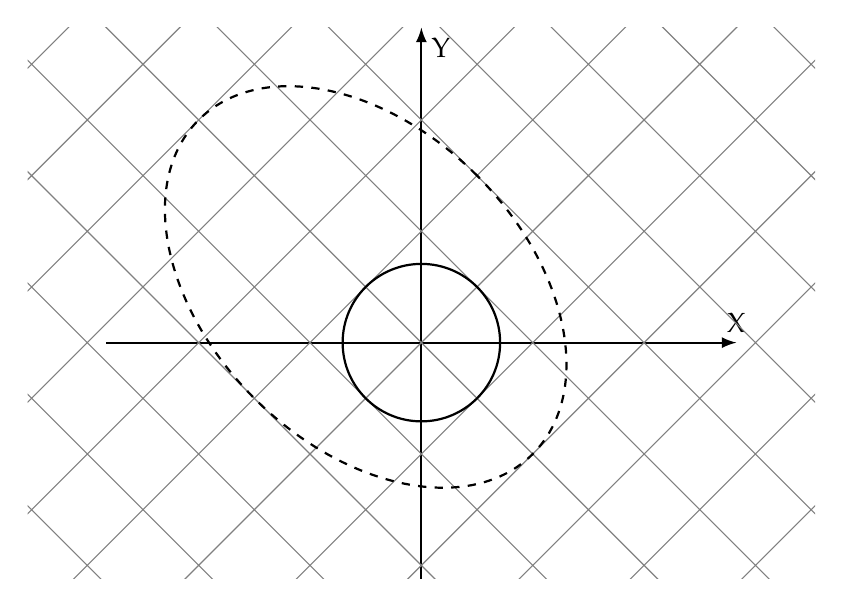
\begin{tikzpicture}
    \path[clip] (-5,-3) rectangle (5,4);
    \draw[axis] (-4,0) -- (4,0) node[anchor=south] {X};
    \draw[axis] (0,-4) -- (0,4) node[anchor=north west] {Y};
    \draw[thin,gray,rotate=45] (-8,-8) grid (8,8);

    \draw[thick] (0,0) circle (1);

    \draw[dashed,thick,rotate=45] (0,1) circle [x radius=2,y radius=3];
  \end{tikzpicture}
\end{center}
\begin{solution}
\[
  M =
  \left[
    \begin{array}{ccc}
      \cos(-45\degrees) & -\sin(-45\degrees) & 0 \\
      \sin(-45\degrees) & \cos(-45\degrees) & 0 \\
      0 & 0 & 1
    \end{array}
  \right]
  \cdot
  \left[
    \begin{array}{ccc}
      1 & 0 & -1 \\
      0 & 1 & 0 \\
      0 & 0 & 1
    \end{array}
  \right]
  \cdot
  \left[
    \begin{array}{ccc}
      3 & 0 & 0 \\
      0 & 2 & 0 \\
      0 & 0 & 1
    \end{array}
  \right]
\]
\[
  M^{-1} =
  \left[
    \begin{array}{ccc}
      1/3 & 0 & 0 \\
      0 & 1/2 & 0 \\
      0 & 0 & 1
    \end{array}
  \right]
  \cdot
  \left[
    \begin{array}{ccc}
      1 & 0 & 1 \\
      0 & 1 & 0 \\
      0 & 0 & 1
    \end{array}
  \right]
  \cdot
  \left[
    \begin{array}{ccc}
      \cos(45\degrees) & -\sin(45\degrees) & 0 \\
      \sin(45\degrees) & \cos(45\degrees) & 0 \\
      0 & 0 & 1
    \end{array}
  \right]
\]
\end{solution}
\end{Exercise}

\begin{Exercise}
Which transformation matrices transform the solid shape $S_1$ into the dashed shape $S_2$ and back?
In other words, find the matrices $A$ and $B$ such that
\[
  A \cdot S_1 = S_2 \qquad B \cdot S_2 = S_1
\]
Write $A$ and $B$ as multiplications of basic transformation matrices (translation, scaling, rotation).
The grid is tilted 30\degrees. Use it to help you determine the exact size of the shapes.
\begin{center}
  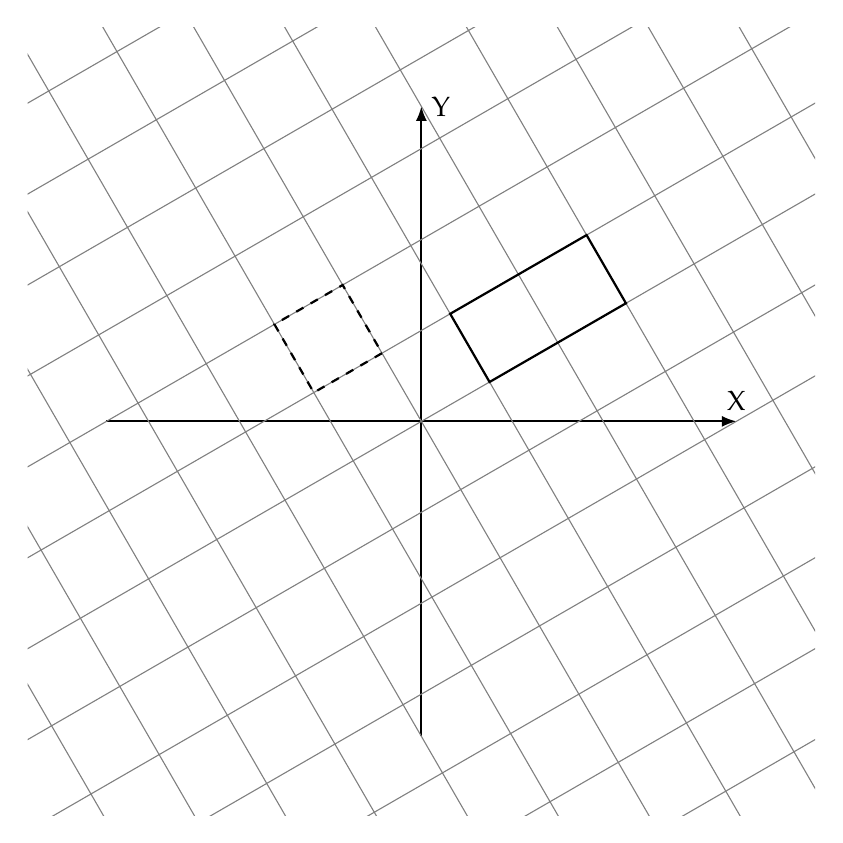
\begin{tikzpicture}
    \path[clip] (-5,-5) rectangle (5,5);
    \draw[axis] (-4,0) -- (4,0) node[anchor=south] {X};
    \draw[axis] (0,-4) -- (0,4) node[anchor=west] {Y};
    \draw[thin,gray,rotate=30] (-8,-8) grid (8,8);

    \begin{scope}[rotate=30]
      \draw[thick] (1,0) rectangle ++(2,1);
    \end{scope}

    \begin{scope}[rotate=120]
      \draw[thick,dashed] (1,0) rectangle ++(1,1);
    \end{scope}
  \end{tikzpicture}
\end{center}
\begin{solution}
\[
  M = \mathrm{Rot}[30\degrees] \cdot \mathrm{Tr}[-1,1] \cdot \mathrm{Sc}[\frac12,1] \cdot \mathrm{Tr}[-1,0] \cdot \mathrm{Rot}[-30\degrees]
\]
\[
  M^{-1} = \mathrm{Rot}[30\degrees] \cdot \mathrm{Tr}[1,0] \cdot \mathrm{Sc}[2,1] \cdot \mathrm{Tr}[1,-1] \cdot \mathrm{Rot}[-30\degrees]
\]
Has to be written down in matrix form on the exam, but using shorthand notation first can help.
\end{solution}
\end{Exercise}

\begin{Exercise}
Find two ways to transform the solid shape $S_1$ into the dashed shape $S_2$.
Give also the inverse transformations.
In other words, find two matrices $A$ and $B$ such that
\[
  A \cdot S_1 = S_2 \qquad B \cdot S_1 = S_2
\]
Write $A$ and $B$ and their inverse matrices $A^{-1}$ and $B^{-1}$ as multiplications of basic
transformation matrices (translation, scaling, rotation).
\begin{center}
  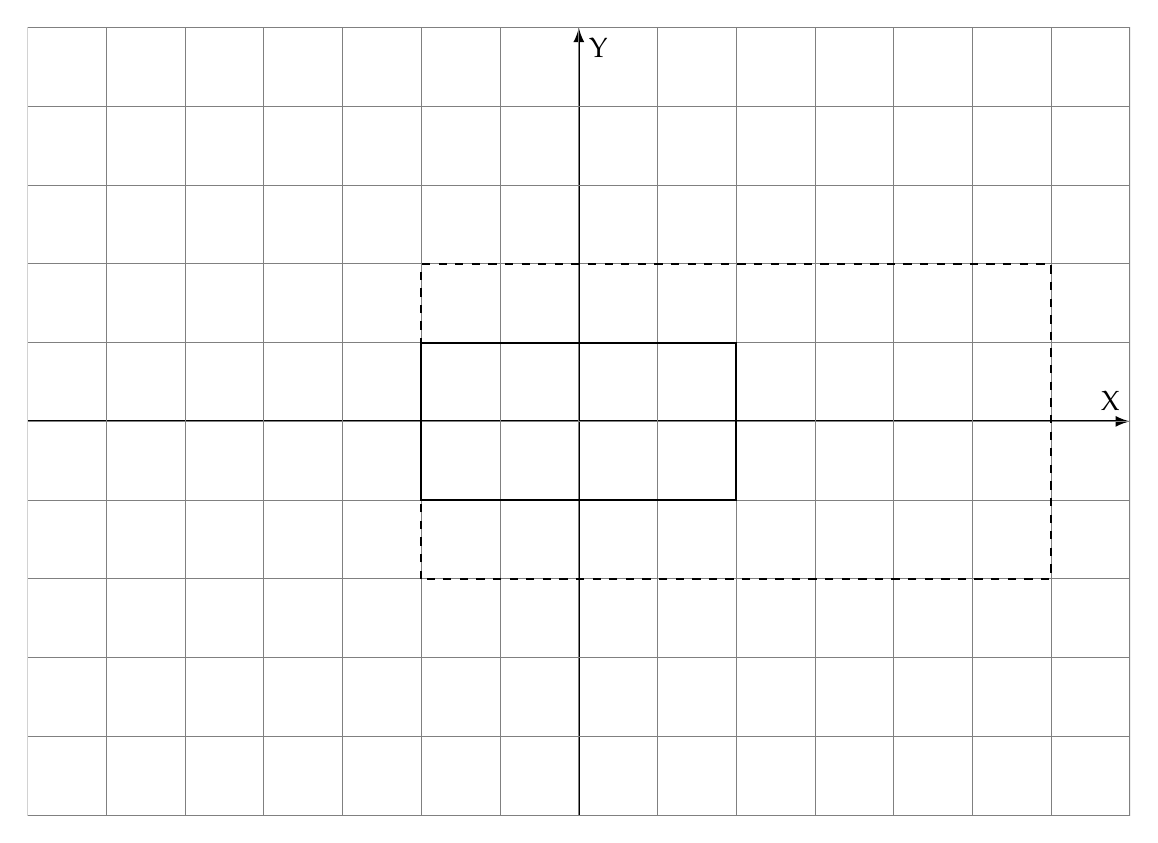
\begin{tikzpicture}
    \path[clip] (-7,-5) rectangle (7,5);
    \draw[axis] (-7,0) -- (7,0) node[anchor=south east] {X};
    \draw[axis] (0,-5) -- (0,5) node[anchor=north west] {Y};

    \draw[thin,gray] (-8,-8) grid (8,8);

    \begin{scope}[]
      \draw[thick] (-2,-1) rectangle ++(4,2);
    \end{scope}

    \begin{scope}[xshift=2cm,scale=2]
      \draw[thick,dashed] (-2,-1) rectangle ++(4,2);
    \end{scope}
  \end{tikzpicture}
\end{center}
\begin{solution}
\[
  A = \mathrm{Tr}[2,0] \cdot \mathrm{Sc}[2,2] \qquad B = \mathrm{Sc}[2,2] \cdot \mathrm{Tr}[1,0]
\]
\[
  A^{-1} = \mathrm{Sc}[\frac12,\frac12] \cdot \mathrm{Tr}[-2,0] \qquad B^{-1} = \mathrm{Tr}[-1,0] \cdot \mathrm{Sc}[\frac12,\frac12]
\]
Has to be written down in matrix form on the exam, but using shorthand notation first can help.
\end{solution}
\end{Exercise}

\begin{Exercise}
Say we have the (rather silly) idea of using quaternions for 2D rotation. Write down the formula
to perform the 2D rotation shown below using quaternions.
\begin{center}
  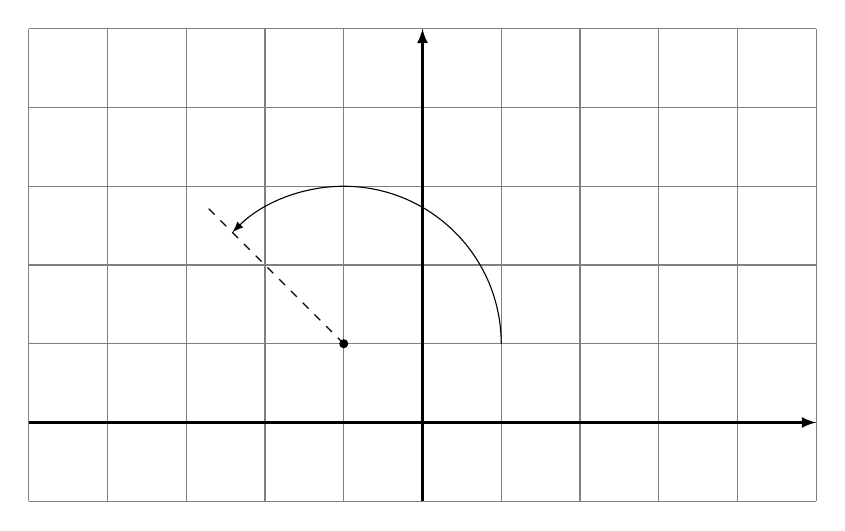
\begin{tikzpicture}
    \draw[thin,black!50] (-5,-1) grid (5,5);
    \draw[axis] (-5,0) -- (5,0);
    \draw[axis] (0,-1) -- (0,5);

    \begin{scope}[xshift=-1cm,yshift=1cm]
      \draw[fill=black] (0,0) circle [radius=0.05];
      \draw[-latex] (2,0) arc [radius=2,start angle=0,delta angle=135];
      \draw[dashed] (0,0) -- (135:2.5);
    \end{scope}
  \end{tikzpicture}
\end{center}
\begin{solution}
\begin{itemize}
  \item Quaternions work in 3D, so we should see this as a rotation around the Z-axis which is perpendicular on the XY plane.
    The Z-axis is represented by the vector $(0,0,1)$.
  \item Rotation is not around the origin, so we need to introduce a pre- and posttranslation represented by
    the vectors $(1,-1,0)$ and $(-1,1,0)$.
  \item The angle $\theta$ by which to rotate is 135\degrees.
  \item The point to be rotated is $(1,1,0)$.
\end{itemize}
This gives us
\[
  \begin{array}{rcl}
    q & = & \cos(67.5\degrees) + \sin(67.5\degrees) \; k \\
    \conj q & = & \cos(67.5\degrees) - \sin(67.5\degrees) \; k \\
    p & = & 2i \\
    x' i + y' j + z' k & = & q \cdot p \cdot \conj q \\
  \end{array}
\]
The rotation of the point $(1,1,0)$ around the Z-axis through $(-1,1,0)$ is $(x'-1,y'+1,z')$.
\end{solution}
\end{Exercise}

\begin{Exercise}
What is the inverse of the following matrix?
\[
  \left[
    \begin{array}{cccc}
      1 & 0 & 0 & 0 \\
      0 & 1 & 0 & 0 \\
      0 & 0 & 1 & 0 \\
      0 & 0 & 0 & 1 \\
    \end{array}
  \right]
\]
\begin{solution}
This is clearly the identity matrix which does not perform
any transformations at all. The inverse of a no-operation
is a no-operation.
\[
  \left[
    \begin{array}{cccc}
      1 & 0 & 0 & 0 \\
      0 & 1 & 0 & 0 \\
      0 & 0 & 1 & 0 \\
      0 & 0 & 0 & 1 \\
    \end{array}
  \right]
\]
\end{solution}
\end{Exercise}



%%% Local Variables:
%%% mode: latex
%%% TeX-master: "model-exam"
%%% End:

\chapter{Physics}
\section{Lighting Models}
\begin{Definition}[point light]
A \emph{point light} is fully defined by its position $P$ and its intensity $I$.
\end{Definition}

\begin{Definition}[ambient lighting] \index{ambient lighting}\index{lighting!ambient}
Given
\begin{itemize}
  \item an object made out of a material that is characterised by an ambient reflection coefficient $\rho_\+a$,
  \item a light ray with intensity $I$ that hits the object at a point $P$,
  \item an eye positioned at point $E$,
\end{itemize}
then the amount of light reflected by the object at $P$ toward $E$ equals
\[
  \rho_\+a \; I
\]
\end{Definition}

\begin{extra}
  \begin{example}
  We split the material's reflection coefficient into RGB-components:
  \[
    \rho_{\+a,\R} = 0.5 \qquad \rho_{\+a,\G} = 0.1 \qquad \rho_{\+a, \B} = 0.9
  \]
  Say the light has intensity
  \[
    I_\R = 1 \qquad I_\G = 0.5 \qquad I_\B = 0
  \]
  The material then reflects light with intensity (0.5, 0.05, 0).
  \end{example}
\end{extra}

\begin{Definition}[diffuse lighting] \index{diffuse lighting}\index{lighting!diffuse}
Given
\begin{itemize}
  \item an object made of a material that is characterised by a diffuse reflection coefficient $\rho_\+d$,
  \item a light ray that hits an object at position $P$,
  \item an eye positioned at point $E$,
\end{itemize}
then the amount of light reflected toward $E$ equals
\[
  \rho_\+d \; I \; \cos\theta
\]
where $\theta$ is the angle between the normal vector on the surface of the object at $P$ and
the incoming light ray.
\begin{center}
  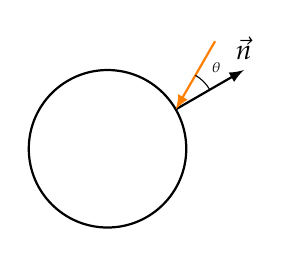
\begin{tikzpicture}
    \draw[thick] (0,0) circle (1);
    \draw[vector] (30:1) -- (30:2) node[at end,anchor=south] {$\vec n$};
    \draw[light] (30:1) +(60:1) -- (30:1);
    \draw (30:1.5) arc[start angle=30,end angle=60,radius=0.5] node[midway,font=\tiny,anchor=south west,inner sep=1mm] {$\theta$};
  \end{tikzpicture}
\end{center}
\end{Definition}

\begin{extra}
  \begin{example}
  \begin{center}
    \begin{tikzpicture}
      \coordinate (L) at (1,3);
      \coordinate (H) at (0,0);
      \coordinate (N) at (45:1);

      \draw[thick] (-2,2) -- (2,-2);
      \draw[vector] (H) -- (N) node[above] {$\vec n$};
      \point[/point/label=L,/point/position=(L)]
      \point[/point/label=H,/point/anchor=north east,/point/position=(H)]

      \draw[light] (L) -- (H);
      \tikzmath{
        real \a;
        \a = atan2(3,1);
      }
      \draw (45:0.5) arc [start angle=45,end angle=\a,radius=0.5cm,font=\tiny] node[anchor=south west,inner sep=1pt,midway] {$\scriptstyle\theta$};
    \end{tikzpicture}
  \end{center}
  with
  \[
    \begin{array}{r@{\;}c@{\;}l}
      I & = & \colorrgb{1}{0.75}{0} \\
      \rho_\+d & = & \colorrgb{1}{0.5}{1} \\[2mm]
      L & = & (1,3,0) \\
      H & = & (0,0,0) \\
      \vec n & = & (0.707107,0.707107,0) \\
    \end{array}
  \]
  The angle $\theta$ can be found with
  \[
    \cos\theta = \vec n \cdot \frac{L-H}{\norm{L-H}} = 0.894
  \]
  which means that due to the incident angle the object will
  be illuminated at 89.4\% of the light's total brightness.
  Of these 89.4\%, only part is reflected by the object's material.
  Exactly how much is determined is determined by $\rho_\+d$.
  \[
    I \cdot \rho_\+d \cdot \cos\theta = (1 \cdot 1 \cdot 0.894, 0.75 \cdot 0.5 \cdot 0.894, 0 \cdot 1 \cdot 0.894) = (0.894,0.335,0)
  \]
  \end{example}
\end{extra}

\begin{Definition}[specular lighting] \index{specular lighting}\index{lighting!specular}
Given
\begin{itemize}
  \item an object made of a material that is characterised by  a specular reflection
        coefficient $\rho_\+d$ and a phong exponent $e$,
  \item a light ray that hits an object at position $P$,
  \item an eye positioned at point $E$,
\end{itemize}
then the amount of light reflected toward $E$ equals
\[
  \rho_\+s \; I \; (\cos\theta)^e
\]
where $\theta$ is the angle between the reflection of the light ray on the surface of the object at $P$ and
the vector $\overrightarrow{PE}$.
\begin{center}
  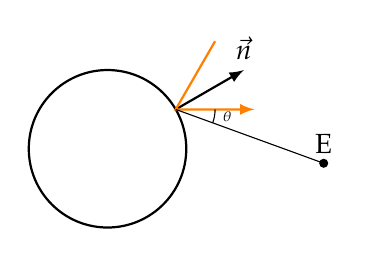
\begin{tikzpicture}
    \coordinate (P) at (30:1);
    \coordinate (eye) at ($ (P) + (-20:2) $);
    \draw[thick] (0,0) circle (1);
    \draw[vector] (P) -- (30:2) node[at end,anchor=south] {$\vec n$};
    \draw[light] (P) +(60:1) -- (P) -- ++(0:1);
    \point[/point/label=E,/point/position=(eye)];
    \draw (P) -- (eye);
    \draw (30:1) ++ (0.5,0) arc[start angle=0,end angle=-20,radius=0.5] node[midway,font=\tiny,anchor=west,inner sep=1mm] {$\theta$};
  \end{tikzpicture}
\end{center}
\end{Definition}

\begin{extra}
  \begin{example}
  \begin{center}
    \begin{tikzpicture}
      \coordinate (L) at (1,3);
      \coordinate (R) at (3,1);
      \coordinate (H) at (0,0);
      \coordinate (N) at (45:1);
      \coordinate (E) at (6,0);

      \draw[thick] (-2,2) -- (2,-2);
      \draw[vector] (H) -- (N) node[above] {$\vec n$};
      \point[/point/label=L,/point/position=(L)]
      \point[/point/label=H,/point/anchor=north east,/point/position=(H)]
      \point[/point/label=E,/point/position=(E)]

      \draw[light] (L) -- (H) -- (R);
      \draw (H) -- (E);
      \tikzmath{
        real \a;
        \a = atan2(1,3);
      }
      \draw (0:1) arc [start angle=0,end angle=\a,radius=1cm,font=\tiny] node[anchor=west,inner sep=1pt,midway] {$\scriptstyle\theta$};
    \end{tikzpicture}
  \end{center}
  with
  \[
    \begin{array}{r@{\;}c@{\;}l@{\qquad}r@{\;}c@{\;}l}
      I & = & \colorrgb{1}{0.75}{0} & L & = & (1,3,0) \\
      \rho_\+s & = & \colorrgb{1}{0.5}{1} & H & = & (0,0,0) \\
      e & = & 10 & E & = & (6,0,0) \\
      &&& \vec n & = & (0.707107,0.707107,0) \\
    \end{array}
  \]
  We compute how the light ray is reflected. We reflected vector is $H-L$, the reflecting vector is $\vec n$:
  \[
    \vec{r} = v - 2 \cdot (\vec v \cdot \vec n) \cdot n = (3,1,0)
  \]
  We need the angle between $\vec r$ and $E-H$:
  \[
    \cos\theta=\frac{\vec r}{\norm{\vec r}} \cdot \frac{E-H}{\norm{E-H}} = 0.949
  \]
  We compute the final colour:
  \[
    I \cdot \rho_s \cdot \cos(\theta)^e = (0.592464, 0.222174, 0)
  \]
  \end{example}
\end{extra}


\section{Refraction}
\begin{Definition}[Snell's law] \index{Snell's law} \index{refractive index}
Given a light ray that moves from a medium with refractive index $n_1$
into a medium with refractive index $n_2$, the incoming angle $\theta_\+i$
and $\theta_\+o$ obey the following law:
\[
  n_1 \sin \theta_\+i = n_2 \sin \theta_\+o
\]
\begin{center}
  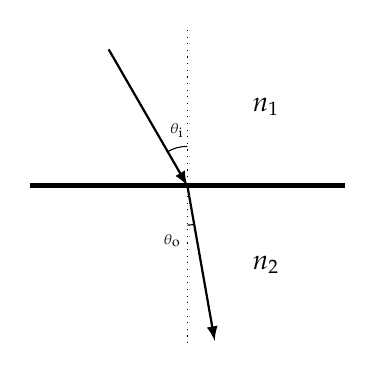
\begin{tikzpicture}
    \draw[ultra thick] (-2,0) -- (2,0);
    \draw[dotted] (0,-2) -- (0,2);
    \draw[vector] (120:2) -- (0,0);
    \draw[vector] (0,0) -- (-80:2);
    \draw (90:0.5) arc [start angle=90,end angle=120,radius=0.5] node[font=\tiny,anchor=south,midway] { $\theta_\+i$ };
    \draw (-80:0.5) arc [start angle=-80,end angle=-90,radius=0.5] node[font=\tiny,anchor=north east,midway] { $\theta_\+o$ };
    \node at (1,1) {$n_1$};
    \node at (1,-1) {$n_2$};
  \end{tikzpicture}
\end{center}
\end{Definition}

\begin{Definition}[refractive indices] \index{refractive index}
The following materials' refractive indices are listed in the table below:
\begin{center}
  \begin{tabular}{rl}
    {\bfseries Material} & {\bfseries Refractive index} \\
    \toprule
    Air \index{air} & 1 \\
    Water \index{water} & 1.33 \\
    Glass \index{glass} & 1.5 \\
    Sapphire \index{sapphire} & 1.77 \\
    Diamond \index{diamond} & 2.42 \\
  \end{tabular}
\end{center}
\end{Definition}

\begin{Definition}[total internal reflection] \index{total internal reflection}
\emph{Total internal reflection} occurs when
\[
  \frac{n_1}{n_2} \sin \theta_\+i > 1
\]
In this case, the light ray is not refracted but reflected.
\end{Definition}

\begin{samepage}
\begin{theorem}\label{thm:vectorial-refraction}
Given
\begin{itemize}
  \item a light ray that moves in a direction described by the unit vector $\vec v$, and
  \item this light ray moves from a medium with refractive index $n_1$ into a medium with refractive index $n_2$, and
  \item $\vec n$ is the normal vector on the surface separating both mediums at the position where
        the light ray hits this surface,
\end{itemize}
\begin{center}
  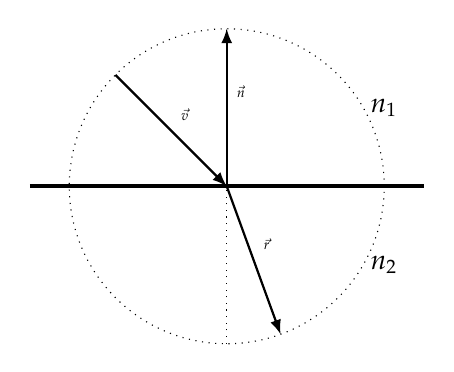
\begin{tikzpicture}
    \draw[ultra thick] (-2.5,0) -- (2.5,0);
    \draw[dotted] (0,-2) -- (0,2);
    \draw[vector] (135:2) -- (0,0) node[midway,anchor=south west,font=\tiny] {$\vec v$};
    \draw[vector] (0,0) -- (-70:2) node[midway,anchor=south west,font=\tiny] {$\vec r$};
    \draw[vector] (0,0) -- (90:2) node[midway,anchor=south west,font=\tiny] {$\vec n$};
    \node at (2,1) {$n_1$};
    \node at (2,-1) {$n_2$};
    \draw[dotted,thin] (0,0) circle (2);
  \end{tikzpicture}
\end{center}
Then the direction of the refracted light ray can be found by computing
\[
  \begin{array}{r@{\;}c@{\;}l}
    \vec r_\+x & = & \displaystyle \frac{n_1}{n_2} (\vec v - (\vec v \cdot \vec n) \cdot \vec n) \\ \\
    \vec r_\+y & = & -\sqrt{1-\norm{\vec r_\+x}^2} \cdot \vec n \\ \\
    \vec r & = & \vec r_\+x + \vec r_\+y
  \end{array}
\]
\end{theorem}
\end{samepage}
\begin{extra}
  \begin{proof}
  We add a few elements to the sketch:
  \begin{center}
    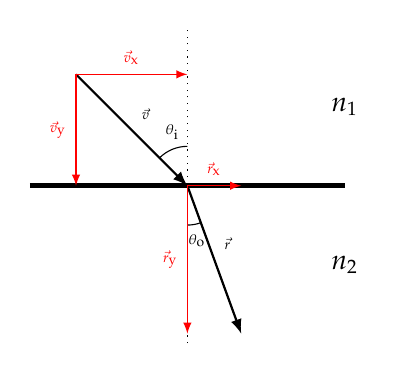
\begin{tikzpicture}
      \draw[ultra thick] (-2,0) -- (2,0);
      \draw[dotted] (0,-2) -- (0,2);
      \draw[vector] (135:2) -- (0,0) node[midway,anchor=south west,font=\tiny] {$\vec v$};
      \draw[vector,thin,red] let \p1=(135:2) in (\p1) -- (0,\y1) node[midway,anchor=south,font=\tiny] {$\vec v_\+x$};
      \draw[vector,thin,red] let \p1=(135:2) in (\p1) -- (\x1,0) node[midway,anchor=east,font=\tiny] {$\vec v_\+y$};
      \draw[vector] (0,0) -- (-70:2) node[midway,anchor=south west,font=\tiny] {$\vec r$};
      \draw (90:0.5) arc [start angle=90,end angle=135,radius=0.5] node[font=\tiny,anchor=south,midway] { $\theta_\+i$ };
      \draw (-70:0.5) arc [start angle=-70,end angle=-90,radius=0.5] node[font=\tiny,anchor=north,midway,xshift=1pt] { $\theta_\+o$ };
      \draw[vector,thin,red] let \p1=(-70:2) in (0,0) -- (\x1,0) node[midway,anchor=south,font=\tiny] {$\vec r_\+x$};
      \draw[vector,thin,red] let \p1=(-70:2) in (0,0) -- (0,\y1) node[midway,anchor=east,font=\tiny] {$\vec r_\+y$};
      \node at (2,1) {$n_1$};
      \node at (2,-1) {$n_2$};
    \end{tikzpicture}
  \end{center}
  From the sketch, we can deduce
  \[
    \begin{array}{r@{\;}c@{\;}l@{\hspace{1cm}}r@{\;}c@{\;}l}
      \norm{\vec v} & = & 1    & \norm{\vec r} & = & 1 \\ \\
      \vec v & = & \vec v_\+x + \vec v_\+y    & \vec r & = & \vec r_\+x + \vec r_\+y \\ \\
      \sin \theta_\+i & = & \displaystyle \frac{\norm{\vec v_\+x}}{\norm{\vec v}} & \sin \theta_\+o & = & \displaystyle \frac{\norm{\vec r_\+x}}{\norm{\vec r}} \\ \\
    \end{array}
  \]
  \[
    n_1 \sin \theta_\+i = n_2 \sin \theta_\+o
  \]
  Our goal is to express $\vec{r}$ in terms of $\vec v$, $\vec n$, $n_1$ and $n_2$.
  We decompose $\vec v$ into $\vec v_\+x$ and $\vec v_\+y$:
  \[
    \vec v_\+y = (\vec v \cdot \vec n) \cdot \vec n \qquad \vec v_\+x = \vec v-\vec v_\+y = \vec v - (\vec v \cdot \vec n) \cdot \vec n
  \]
  We determine $\vec r_\+x$'s length:
  \[
    \norm{\vec r_\+x} = \norm{\vec r} \sin\theta_\+o = \sin\theta_\+o = \frac{n_1}{n_2} \sin \theta_\+i = \frac{n_1}{n_2} \norm{\vec v_\+x}
  \]
  Since $\vec{r}_\+x$ is parallel to $\vec{v}_\+x$ and points in the same direction, we get
  \[
    \vec r_\+x = \frac{n_1}{n_2} \vec v_\+x = \frac{n_1}{n_2} (\vec v - (\vec v \cdot \vec n) \cdot \vec n)
  \]
  We now turn our attention to $\vec r_\+y$.
  \[
    \norm{\vec r_\+x}^2 + \norm{\vec r_\+y}^2 = 1 \qquad\Rightarrow\qquad \norm{\vec r_\+y} = \sqrt{1 - \norm{\vec r_\+x}^2}
  \]
  $\vec r_\+y$ is parallel to $\vec n$:
  \[
    \vec r_\+y = - \sqrt{1 - \norm{\vec r_\+x}^2} \cdot \vec n
  \]
  \end{proof}
\end{extra}

\begin{extra}
  \begin{example}
  \begin{center}
    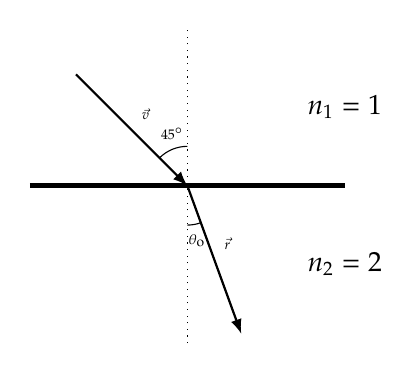
\begin{tikzpicture}
      \draw[ultra thick] (-2,0) -- (2,0);
      \draw[dotted] (0,-2) -- (0,2);
      \draw[vector] (135:2) -- (0,0) node[midway,anchor=south west,font=\tiny] {$\vec v$};
      \draw[vector] (0,0) -- (-70:2) node[midway,anchor=south west,font=\tiny] {$\vec r$};
      \draw (90:0.5) arc [start angle=90,end angle=135,radius=0.5] node[font=\tiny,anchor=south,midway] { $45\degrees$ };
      \draw (-70:0.5) arc [start angle=-70,end angle=-90,radius=0.5] node[font=\tiny,anchor=north,midway,xshift=1pt] { $\theta_\+o$ };
      \node at (2,1) {$n_1 = 1$};
      \node at (2,-1) {$n_2 = 2$};
    \end{tikzpicture}
  \end{center}
  We first compute the outgoing angle $\theta_\+o$ using Schnell's law:
  \[
    \sin 45\degrees = 2 \sin \theta_\+o \qquad\Rightarrow\qquad \theta_\+o = \arcsin\left(\frac{\sin 45\degrees}{2}\right) = 20.7 \degrees
  \]
  We determine $\vec v$'s and $\vec r$'s coordinates:
  \[
    \begin{array}{r@{\;}c@{\;}l@{\;}c@{\;}l}
      \vec v & = & (\cos 45\degrees, -\sin 45\degrees) & = & (0.707, -0.707) \\
      \vec r & = & (\cos (90\degrees-20.7\degrees), -\sin (90\degrees-20.7\degrees)) & = & (0.353, -0.935)
    \end{array}
  \]
  We now check whether the result using \cref{thm:vectorial-refraction} agrees with this.
  \[
    \begin{array}{r@{\;}c@{\;}l@{\;}c@{\;}l}
      \vec r_\+x & = & \displaystyle \frac{n_1}{n_2} (\vec v - (\vec v \cdot \vec n) \cdot \vec n) & = & (0.353,0) \\ \\
      \vec r_\+y & = & -\sqrt{1-\norm{\vec r_\+x}^2} \cdot \vec n & = & (0, -0.935) \\ \\
      \vec r & = & \vec r_\+x + \vec r_\+y & = & (0.353, -0.935)
    \end{array}
  \]
  \end{example}
\end{extra}

%%% Local Variables:
%%% mode: latex
%%% TeX-master: "reference"
%%% End:

\section{Ray Tracer}
\begin{Exercise}
Give the SDL file that produces this result:
\begin{center}
  \includegraphics[height=6cm]{scene.png}
\end{center}
The camera is located at $(0,0,10)$, looks at $(0,0,0)$ and has up-vector $(0,1,0)$.
The sphere in the middle has radius 1; the lower sphere is twice as big.
Make sure not to forget about the following details:
\begin{itemize}
  \item The lights
  \item The material's properties (these do not have to be 100\% correct)
  \item The exact transformations.
\end{itemize}
\begin{solution}
\lstinputlisting[language={}]{scene.sdl}
\end{solution}
\end{Exercise}

\begin{Exercise}
Give the SDL file that produces this result:
\begin{center}
  \includegraphics[height=5cm]{scene2.png}
\end{center}
The camera is located at $(0,0,10)$, looks at $(0,0,0)$ and has up-vector $(0,1,0)$.
Both spheres have radius 1.
Make sure not to forget about the following details:
\begin{itemize}
  \item The lights
  \item The material's properties (these do not have to be 100\% correct)
  \item The exact transformations.
\end{itemize}
\begin{solution}
\lstinputlisting[language={}]{scene2.sdl}
\end{solution}
\end{Exercise}

\begin{Exercise}
Give the SDL file that produces this result:
\begin{center}
  \includegraphics[height=5cm]{scene3.png}
\end{center}
The camera is located at $(0,0,10)$, looks at $(0,0,0)$ and has up-vector $(0,1,0)$.
Both spheres have radius 1.
Make sure not to forget about the following details:
\begin{itemize}
  \item The lights
  \item The material's properties (these do not have to be 100\% correct)
  \item The exact transformations.
\end{itemize}
\begin{solution}
\lstinputlisting[language={}]{scene3.sdl}
\end{solution}
\end{Exercise}

\begin{Exercise}
Give the SDL file that produces this result:
\begin{center}
  \includegraphics[height=5cm]{scene4.png}
\end{center}
The camera is located at $(0,0,10)$, looks at $(0,0,0)$ and has up-vector $(0,1,0)$.
The sphere has radius 1 and is white. A large square is placed behind this sphere.
Make sure not to forget about the following details:
\begin{itemize}
  \item The lights
  \item The material's properties (these do not have to be 100\% correct)
  \item The exact transformations.
\end{itemize}
\begin{solution}
\lstinputlisting[language={}]{scene4.sdl}
\end{solution}
\end{Exercise}


%%% Local Variables:
%%% mode: latex
%%% TeX-master: "model-exam"
%%% End:

\section{Extensions}
\begin{Exercise}
Currently, our ray tracer allows us to specify only one colour to each shape:
a shape is either completely red, or blue, or white, or \dots
Say we want to achieve the following:
\begin{center}
  \includegraphics[width=.5\linewidth]{3d-textures.png}
\end{center}
What changes would you make to the ray tracer?
\end{Exercise}

\begin{Exercise}
Our shapes are perfectly smooth. It might come in handy to give them a rougher surface.
Take for example the bumpy sphere shown below.
\begin{center}
  \includegraphics[width=.5\linewidth]{bumpmapping.png}
\end{center}
What changes would you make to the ray tracer?
\end{Exercise}

\begin{Exercise}
Our ray tracer understands unions of objects, i.e. it is possible to create
a new shape by grouping two shapes together. There are other operations
like this, which yield more interesting results. Below you can see the result
of \emph{intersecting} two spheres to produce a lens.
\begin{center}
  \includegraphics[width=.5\linewidth]{csg.png}
\end{center}
What changes would you make to support intersection?
\end{Exercise}



\end{document}



%%% Local Variables: 
%%% mode: latex
%%% TeX-master: t
%%% End: 
